\documentclass{article}

% \setlength\parindent{0pt}

\usepackage{graphicx}
\graphicspath{{images/}}
\usepackage{amsmath}
\usepackage{hyperref}
\usepackage{float}
\usepackage{cleveref}
\usepackage[comma,authoryear]{natbib}
\usepackage[section]{placeins}

\usepackage[affil-it]{authblk} 
\usepackage{etoolbox}
\usepackage{lmodern}
\usepackage[font=small]{caption}



\begin{document}

\title{SASSI to ESSI conversion: distorted SASSI elements}
\author{Hexiang Wang}
\maketitle

\section{Introduction}\label{sec: introduction}

SASSI, a System for Analysis of Soil-Structure Interaction developed by \citet{Ostadan2007b}, consists of a number of interrelated computer program modules which can be used to solve a wide range of dynamic soil-structure interaction problems in two or three dimensions.
%
A lot of geometric finite element models has been developed based on SASSI. 

%
While RealESSI (Realistic Earthquake-Soil-Structure Interaction) Simulator is a software, hardware and documentation system for high fidelity, high performance, time domain, nonlinear/inelastic, deterministic or probabilistic, 3D, finite element modeling and simulation of earthquake-soil/rock-structure interaction of Infrastructure Objects (Nuclear Facilities, Dams, Bridges, Buildings, \&c.),
%
It will be very useful if these original SASSI geometric models can be transfered into RealESSI models and conduct nonlinear Soil Structure Interaction (SSI) analysis.  

%
A very handy mesh conversion tool \href{https://github.com/hexiang6666/SASSI_converter}{\textbf{SASSI\_converter}} has been developed for this purpose.   
%
With \textbf{SASSI\_converter}, most of SASSI geometric entities (points, elements, fixities, etc) can be directly converted into corresponding ESSI entities.  
%
However, there are three types of distorted SASSI 8 node brick element (figure \ref{Fig:three types of distorted element} ) needed to be handled with special attention. 

Since in SASSI, there are only 7, 6 and 5 nodes (node IDs) consisting of corresponding eight node brick element, respectively.
%
But in RealESSI, the 8 node brick element must contain 8 different node IDs. 
%
The nodes with two different IDs can share the same location. 
%
Therefore, the conversion strategy adopted here is to reproduce some new nodes with different node IDs but has the same coordinates as these distorted nodes. 
%
Then with these reproduced nodes, ESSI 8 node brick element is formed.      

Rigorous numerical tests have been done to confirm the feasibility and validity of this strategy, shown in section \ref{sec:numerical test}.   

\begin{figure}[H]
\begin{center}
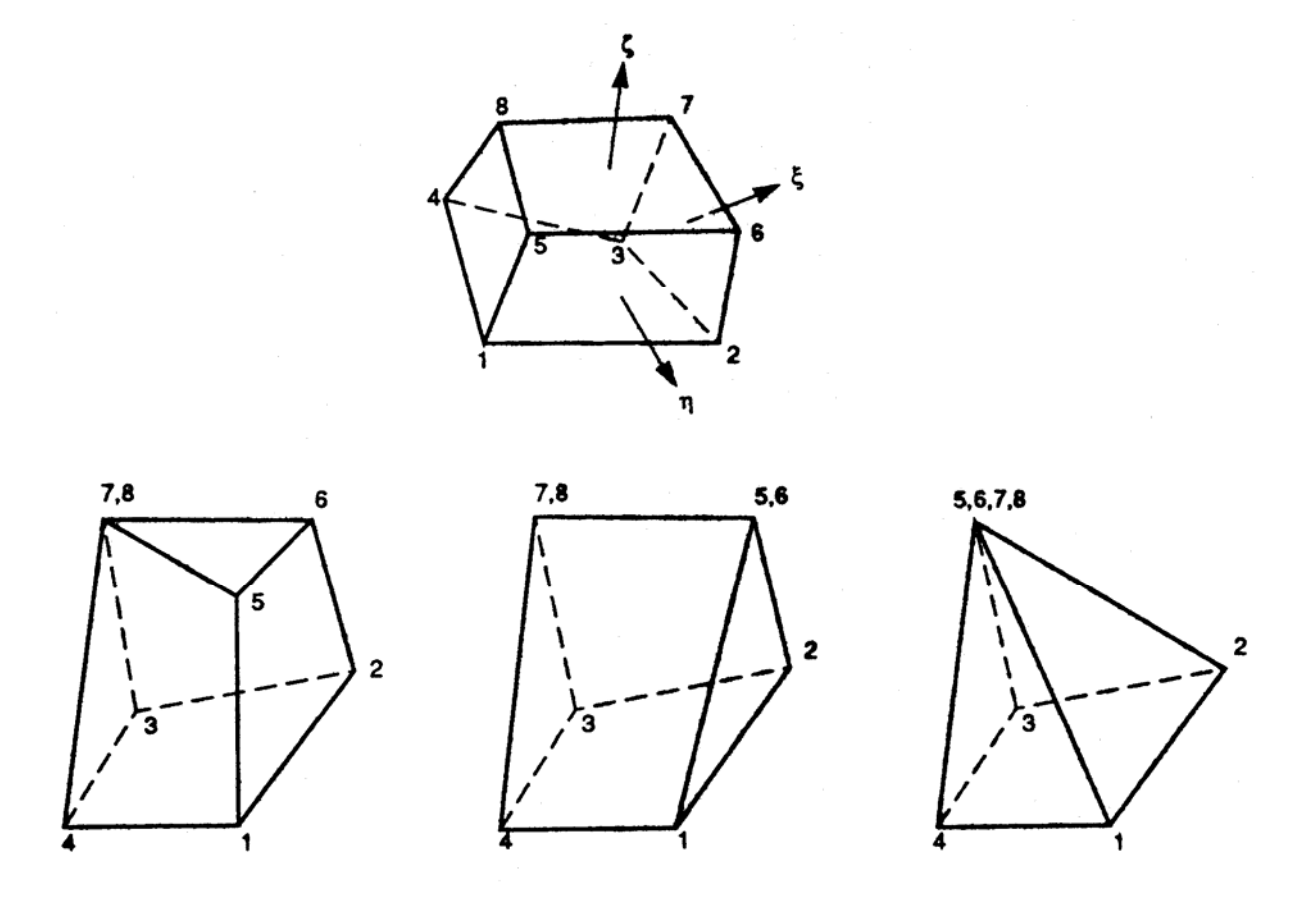
\includegraphics[width=\textwidth]{images/SASSI_distorted_element.png}
\end{center}
\caption{\label{Fig:three types of distorted element} Three types of distorted elements in SASSI}
\end{figure}


\section{Numerical test}\label{sec:numerical test}

\subsection{Test procedure}

With reference to the ``patch test'' put forward by \cite{local-143}, the test procedure is following:

\begin{itemize}
\item 
A standard solution is given by testing two different loading modes on a single normal 8 node brick element:
%
(1) Pure confinment loading, where same pressure are applied on three different directions. 
%
(2) Simple sheaing, where shearing force is applied on four nodes of top layer, while four nodes on bottom layer are totally fixed. 
%
Simple elastic material is adopted here with Young's modulus $E$ as $125\ MPa$ and Poisson's ratio $\mu$ as $0.25$. 
%
The setup of standard test is shown in figure \ref{Fig:setup of standard 8-node element}. 
%
\begin{figure}[H]
\begin{center}
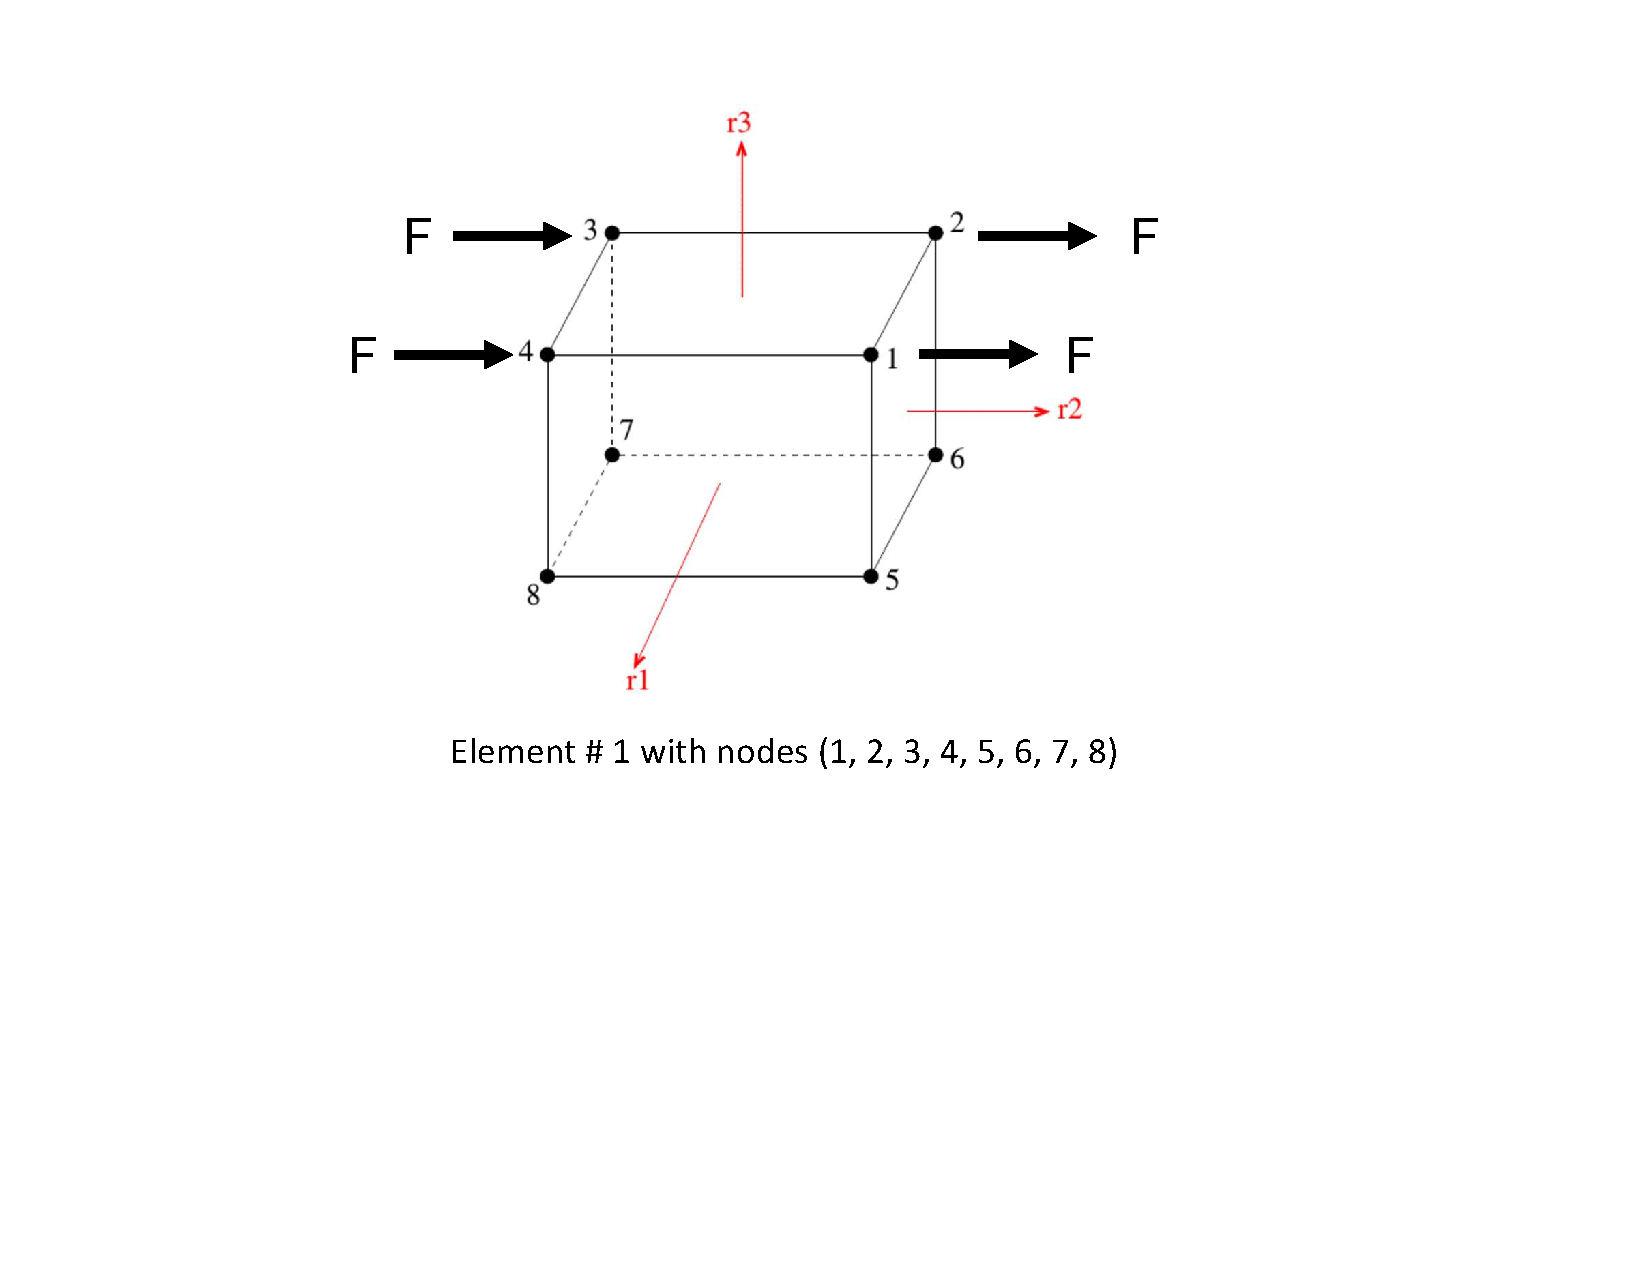
\includegraphics[width=0.6\textwidth]{images/standard_8_node_element.pdf}
\end{center}
\caption{\label{Fig:setup of standard 8-node element} Setup of standard 8-node element}
\end{figure}


% \begin{figure}[H]
% \begin{center}
% 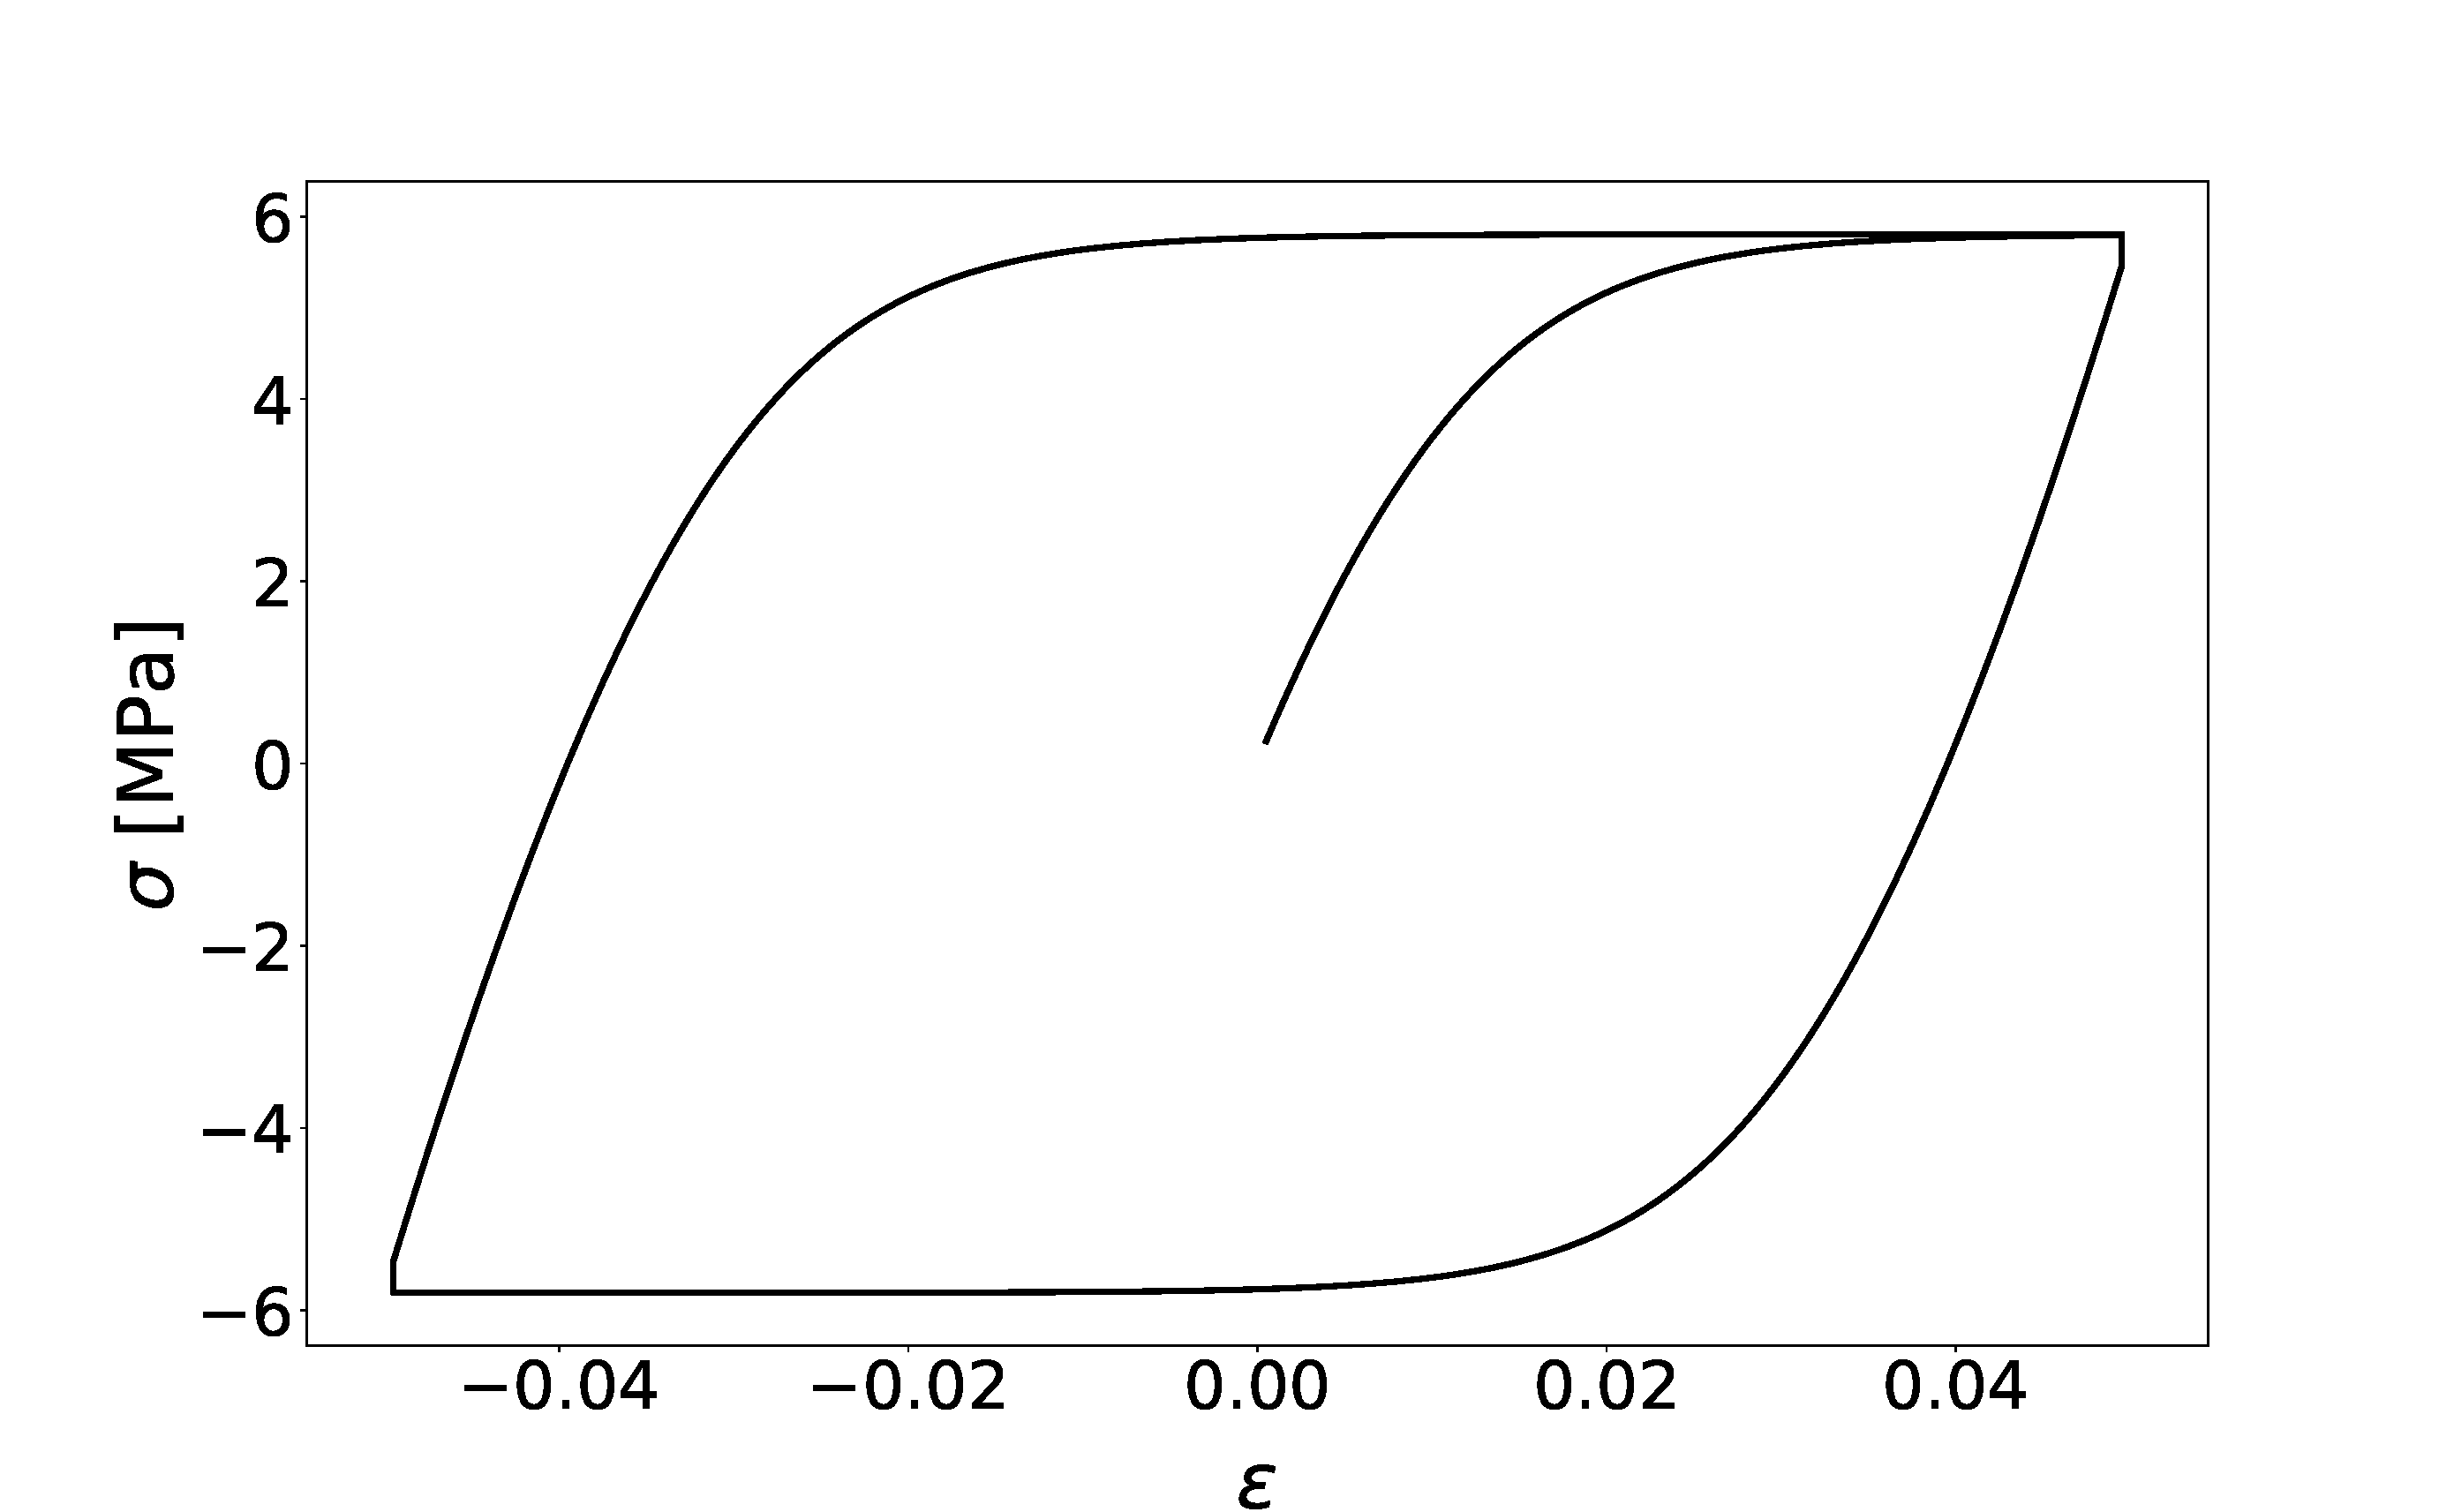
\includegraphics[width=0.6\textwidth]{images/standard_stress_strain.pdf}
% \end{center}
% \caption{\label{Fig:standard stress strain} Stress-strain record of standard 8 node element}
% \end{figure}


%
\item Build the same geometric model with distorted 8 node brick elements and conduct numerical simulation under the same loading and boundary conditions as first step. 

Specifically, the geometric configure for 7-node distorted element is shown in figure \ref{Fig:geometric configuration of numerical test for 7-node distorted element }, where the cubic consists of two 7-node distorted elements. A dummy node 11 is generated at the same location as node 2. 

\begin{figure}[H]
\begin{center}
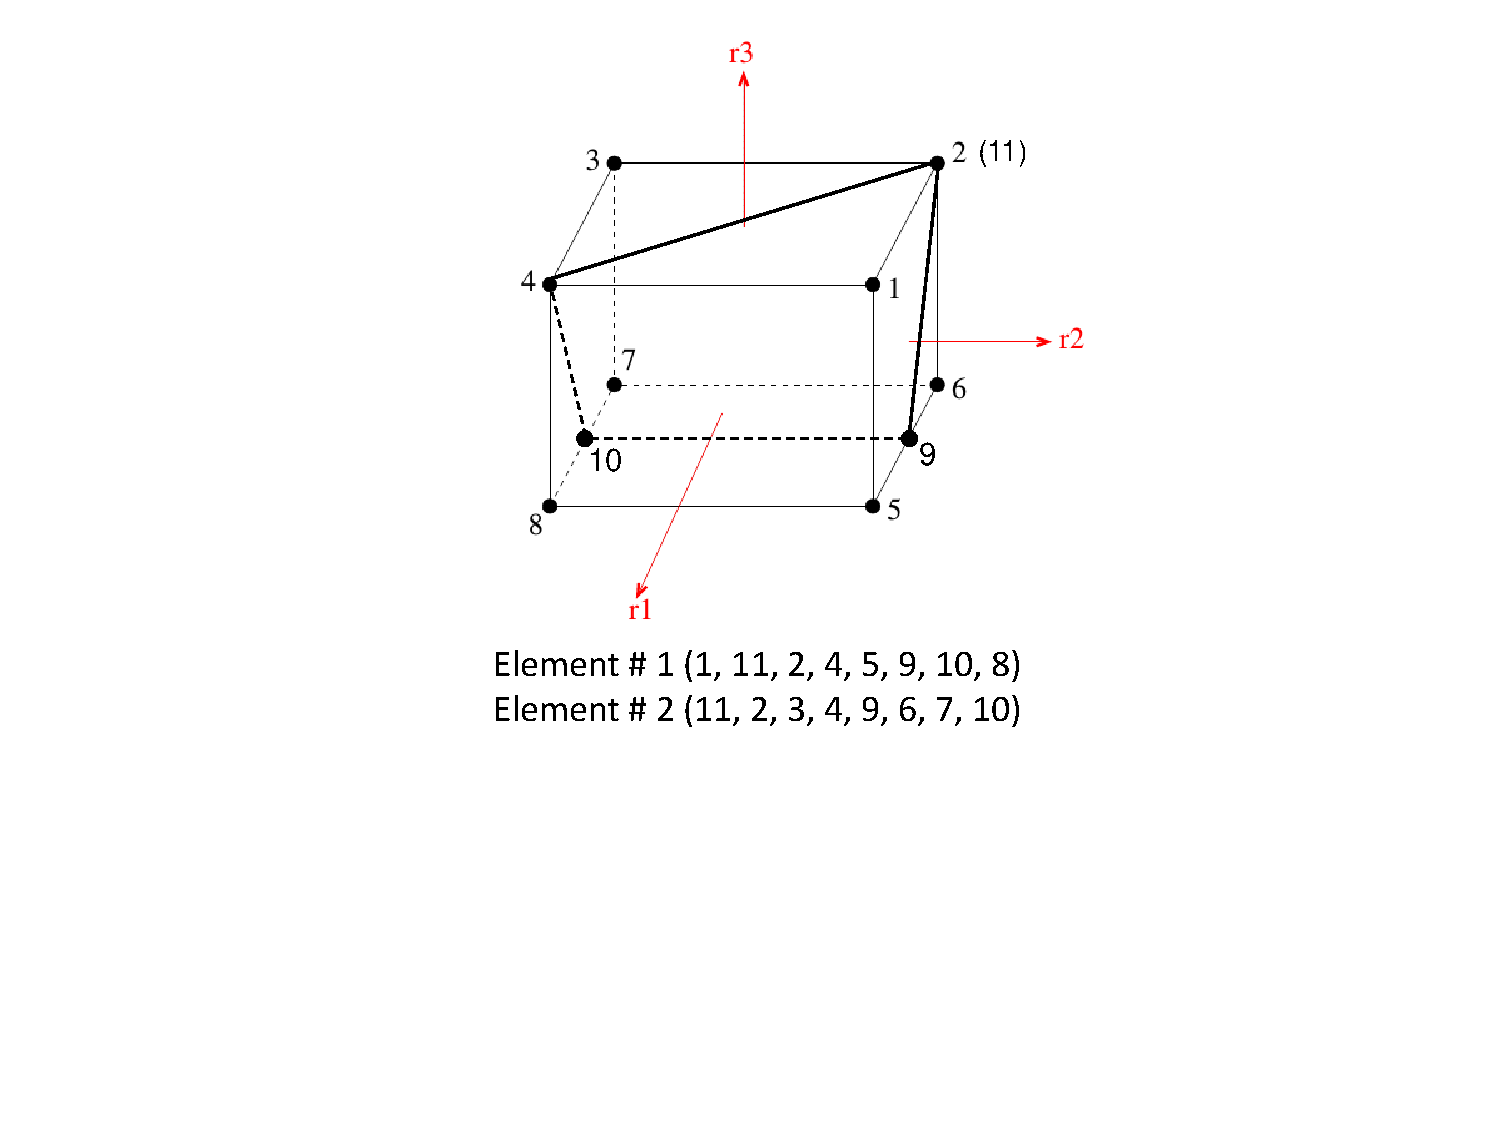
\includegraphics[width=0.4\textwidth]{images/distorted_7_node_element.pdf}
\end{center}
\caption{\label{Fig:geometric configuration of numerical test for 7-node distorted element } Geometric configuration of numerical test for 7-node distorted element}
\end{figure}

The geometric configuration for 6-node distorted element is shown in figure \ref{Fig:geometric configuration of numerical test for 6-node distorted element } .
%
Again the cubic is composed of two 6-node distorted elements. 
%
Two dummy ESSI nodes 9 and 10 are generated at the same location with original node 1 and 2.  

\begin{figure}[H]
\begin{center}
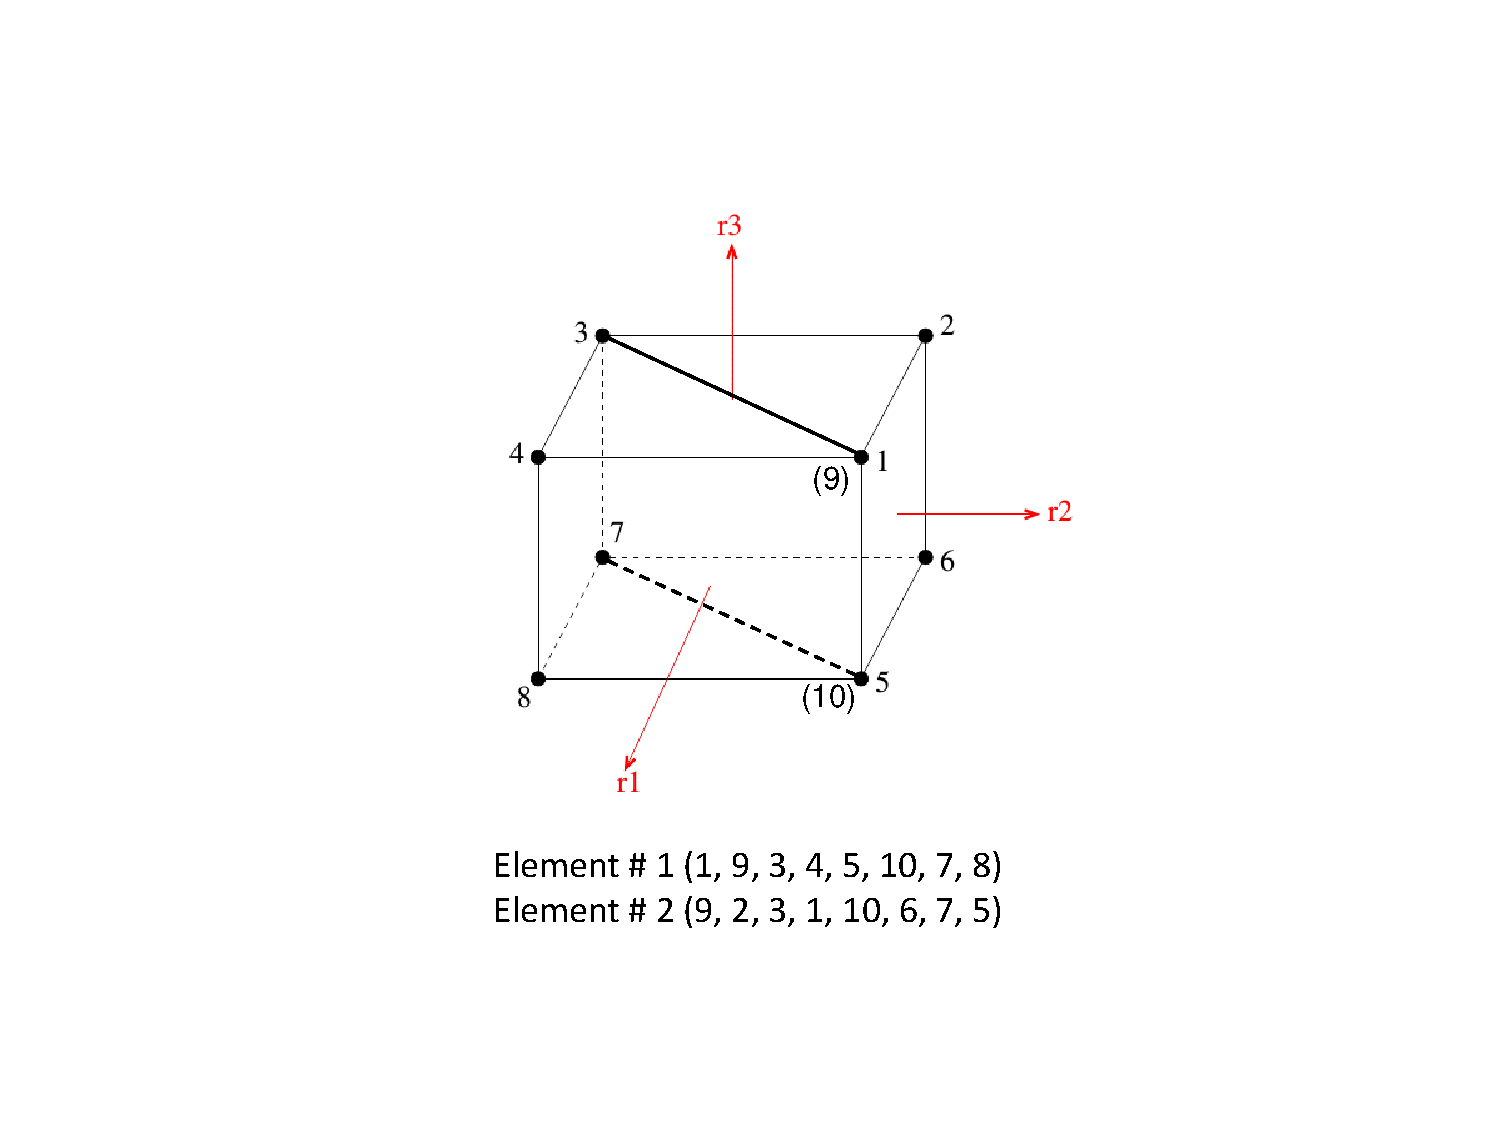
\includegraphics[width=0.4\textwidth]{images/distorted_6_node_element.pdf}
\end{center}
\caption{\label{Fig:geometric configuration of numerical test for 6-node distorted element } Geometric configuration of numerical test for 6-node distorted element}
\end{figure}

%
And figure \ref{Fig:geometric configuration of numerical test for 5-node distorted element } gives the geometric configuration of 5-node distorted element, where the cubic is divided into 3 5-node elements.  

\begin{figure}[H]
\begin{center}
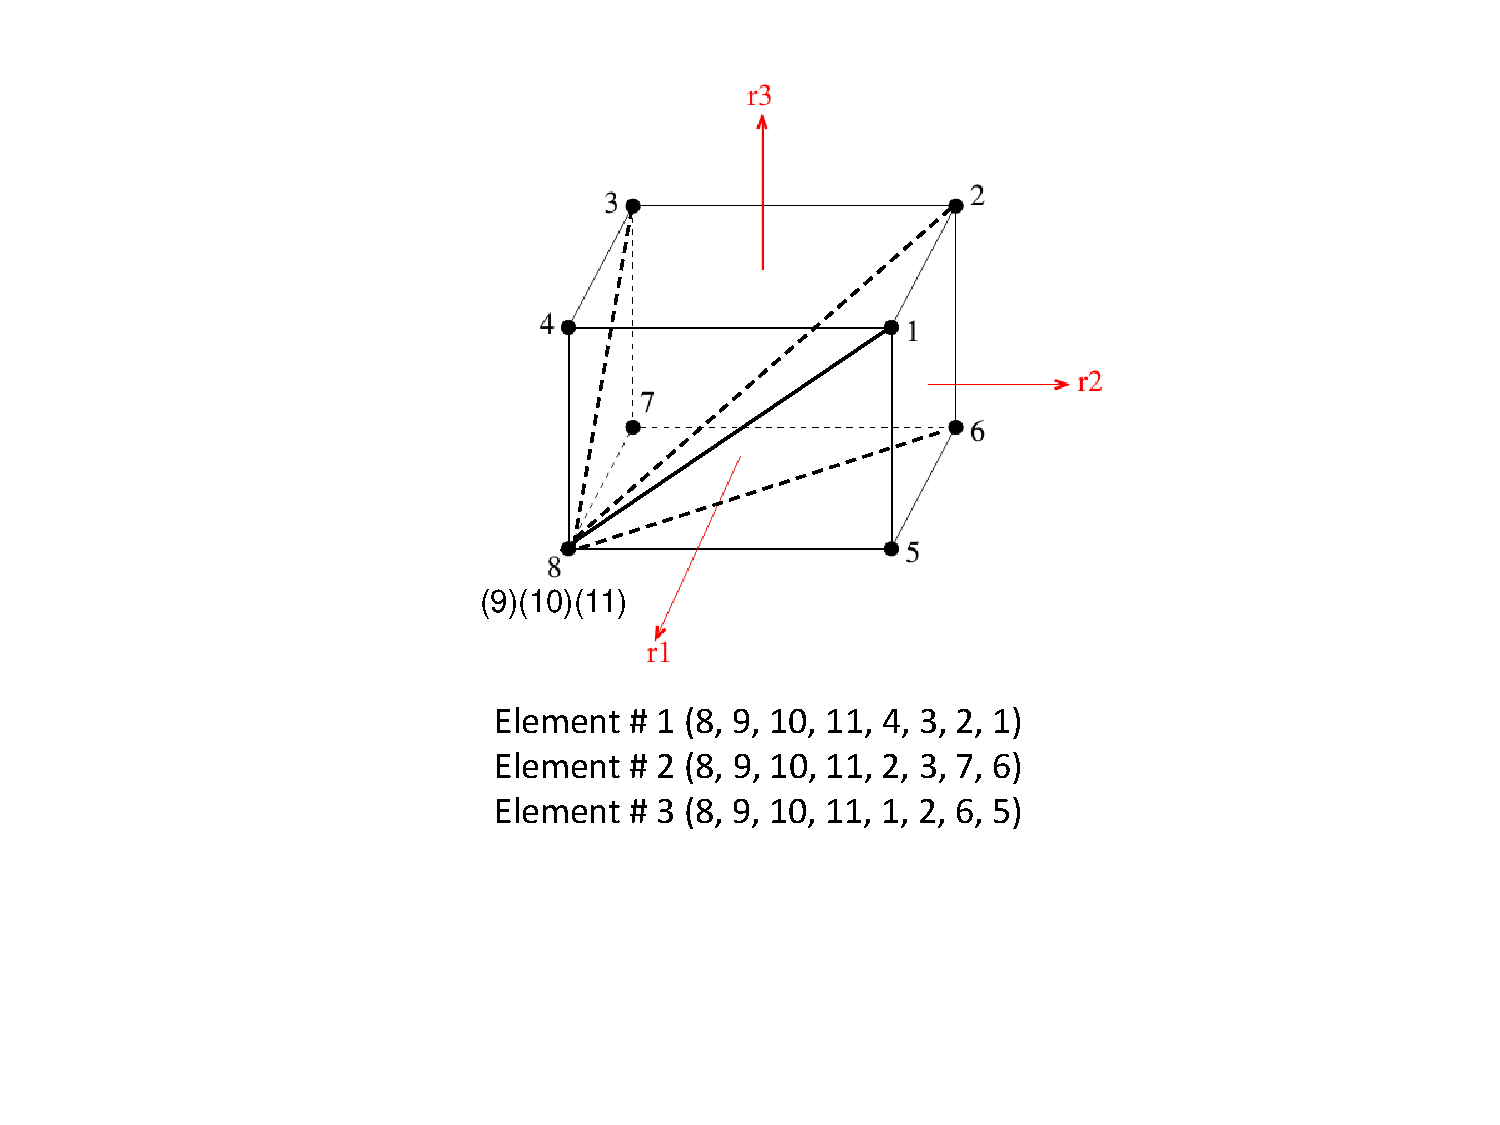
\includegraphics[width=0.4\textwidth]{images/distorted_5_node_element.pdf}
\end{center}
\caption{\label{Fig:geometric configuration of numerical test for 5-node distorted element } Geometric configuration of numerical test for 5-node distorted element}
\end{figure}


%
\item Compare the response of models in step 1 and step 2. If the difference is small enough, the strategy described in section \ref{sec: introduction} is feasible and valid. 
\end{itemize}

\subsection{Test result}

All the input files of numerical tests are placed at the \href{http://cml08.engr.ucdavis.edu/for_professor/distorted_element_test/}{website}. 
%
The comparison of displacement response for confinement loading is shown in figure \ref{Fig: confinement comparison result}. 
%
Figure \ref{Fig: shearing comparison result} demonstrates the test results of simple shearing loading. 
%
It can be seen that the simulation results of these types of distorted element are close to result of standard 8 node brick element. 
%
The line of 6 node distorted element is almost overlap with the line of standard test.
%
Distorted 7-node element and 5-node element experience certain decrease of accuracy. 
%
The main error reflects on the decrease of stiffness. 
%
Both bulk modulus and shear modulus of 7-node element and 5-node element are around 7\% lower than the standard 8-node element.    
%
Therefore, the simulation error of displacement response is proportional to the magnitude of external force. Larger force leads to bigger simulation error.  

% In this particular test, the maximum error happened at the beginning of reloading.
% %
% The solutions of distorted 7-node element and 5-node element is 17\% higher than that of standard 8-node element.     

\begin{figure}[H]
\begin{center}
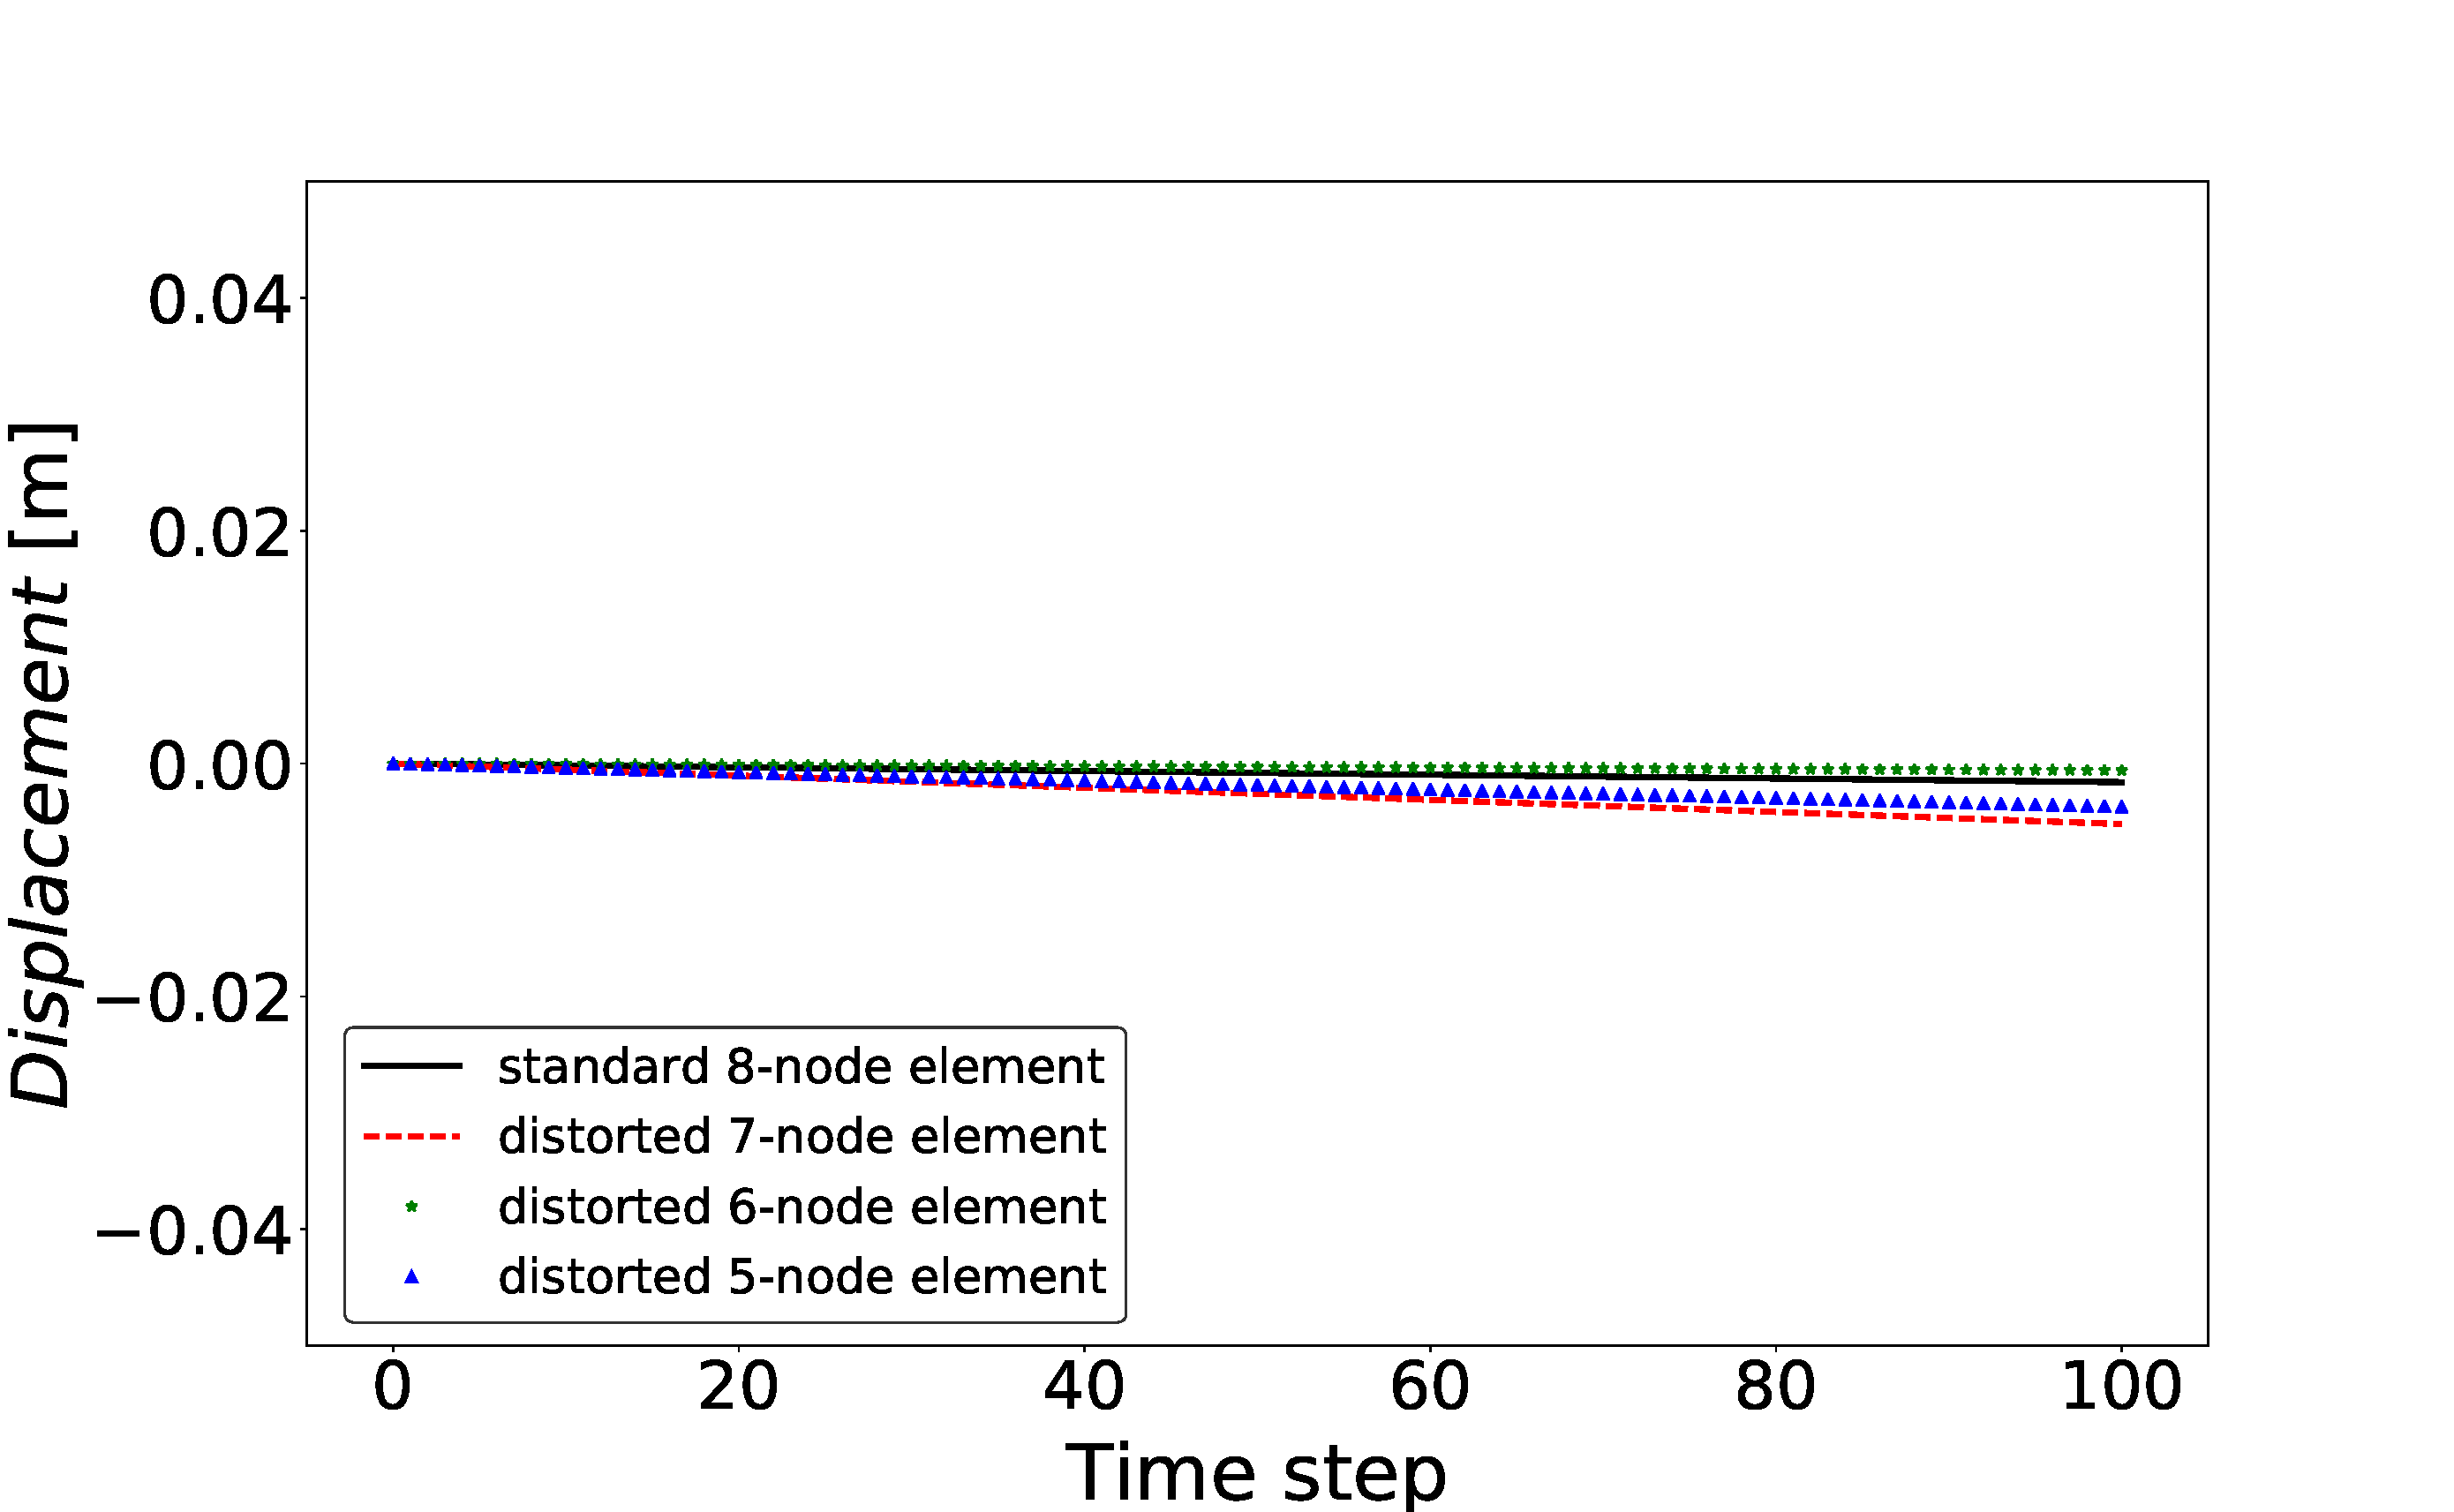
\includegraphics[width=0.8\textwidth]{images/confinement_comparison.pdf}
\end{center}
\caption{\label{Fig: confinement comparison result} Comparison of displacement response under confinement loading}
\end{figure}

\begin{figure}[H]
\begin{center}
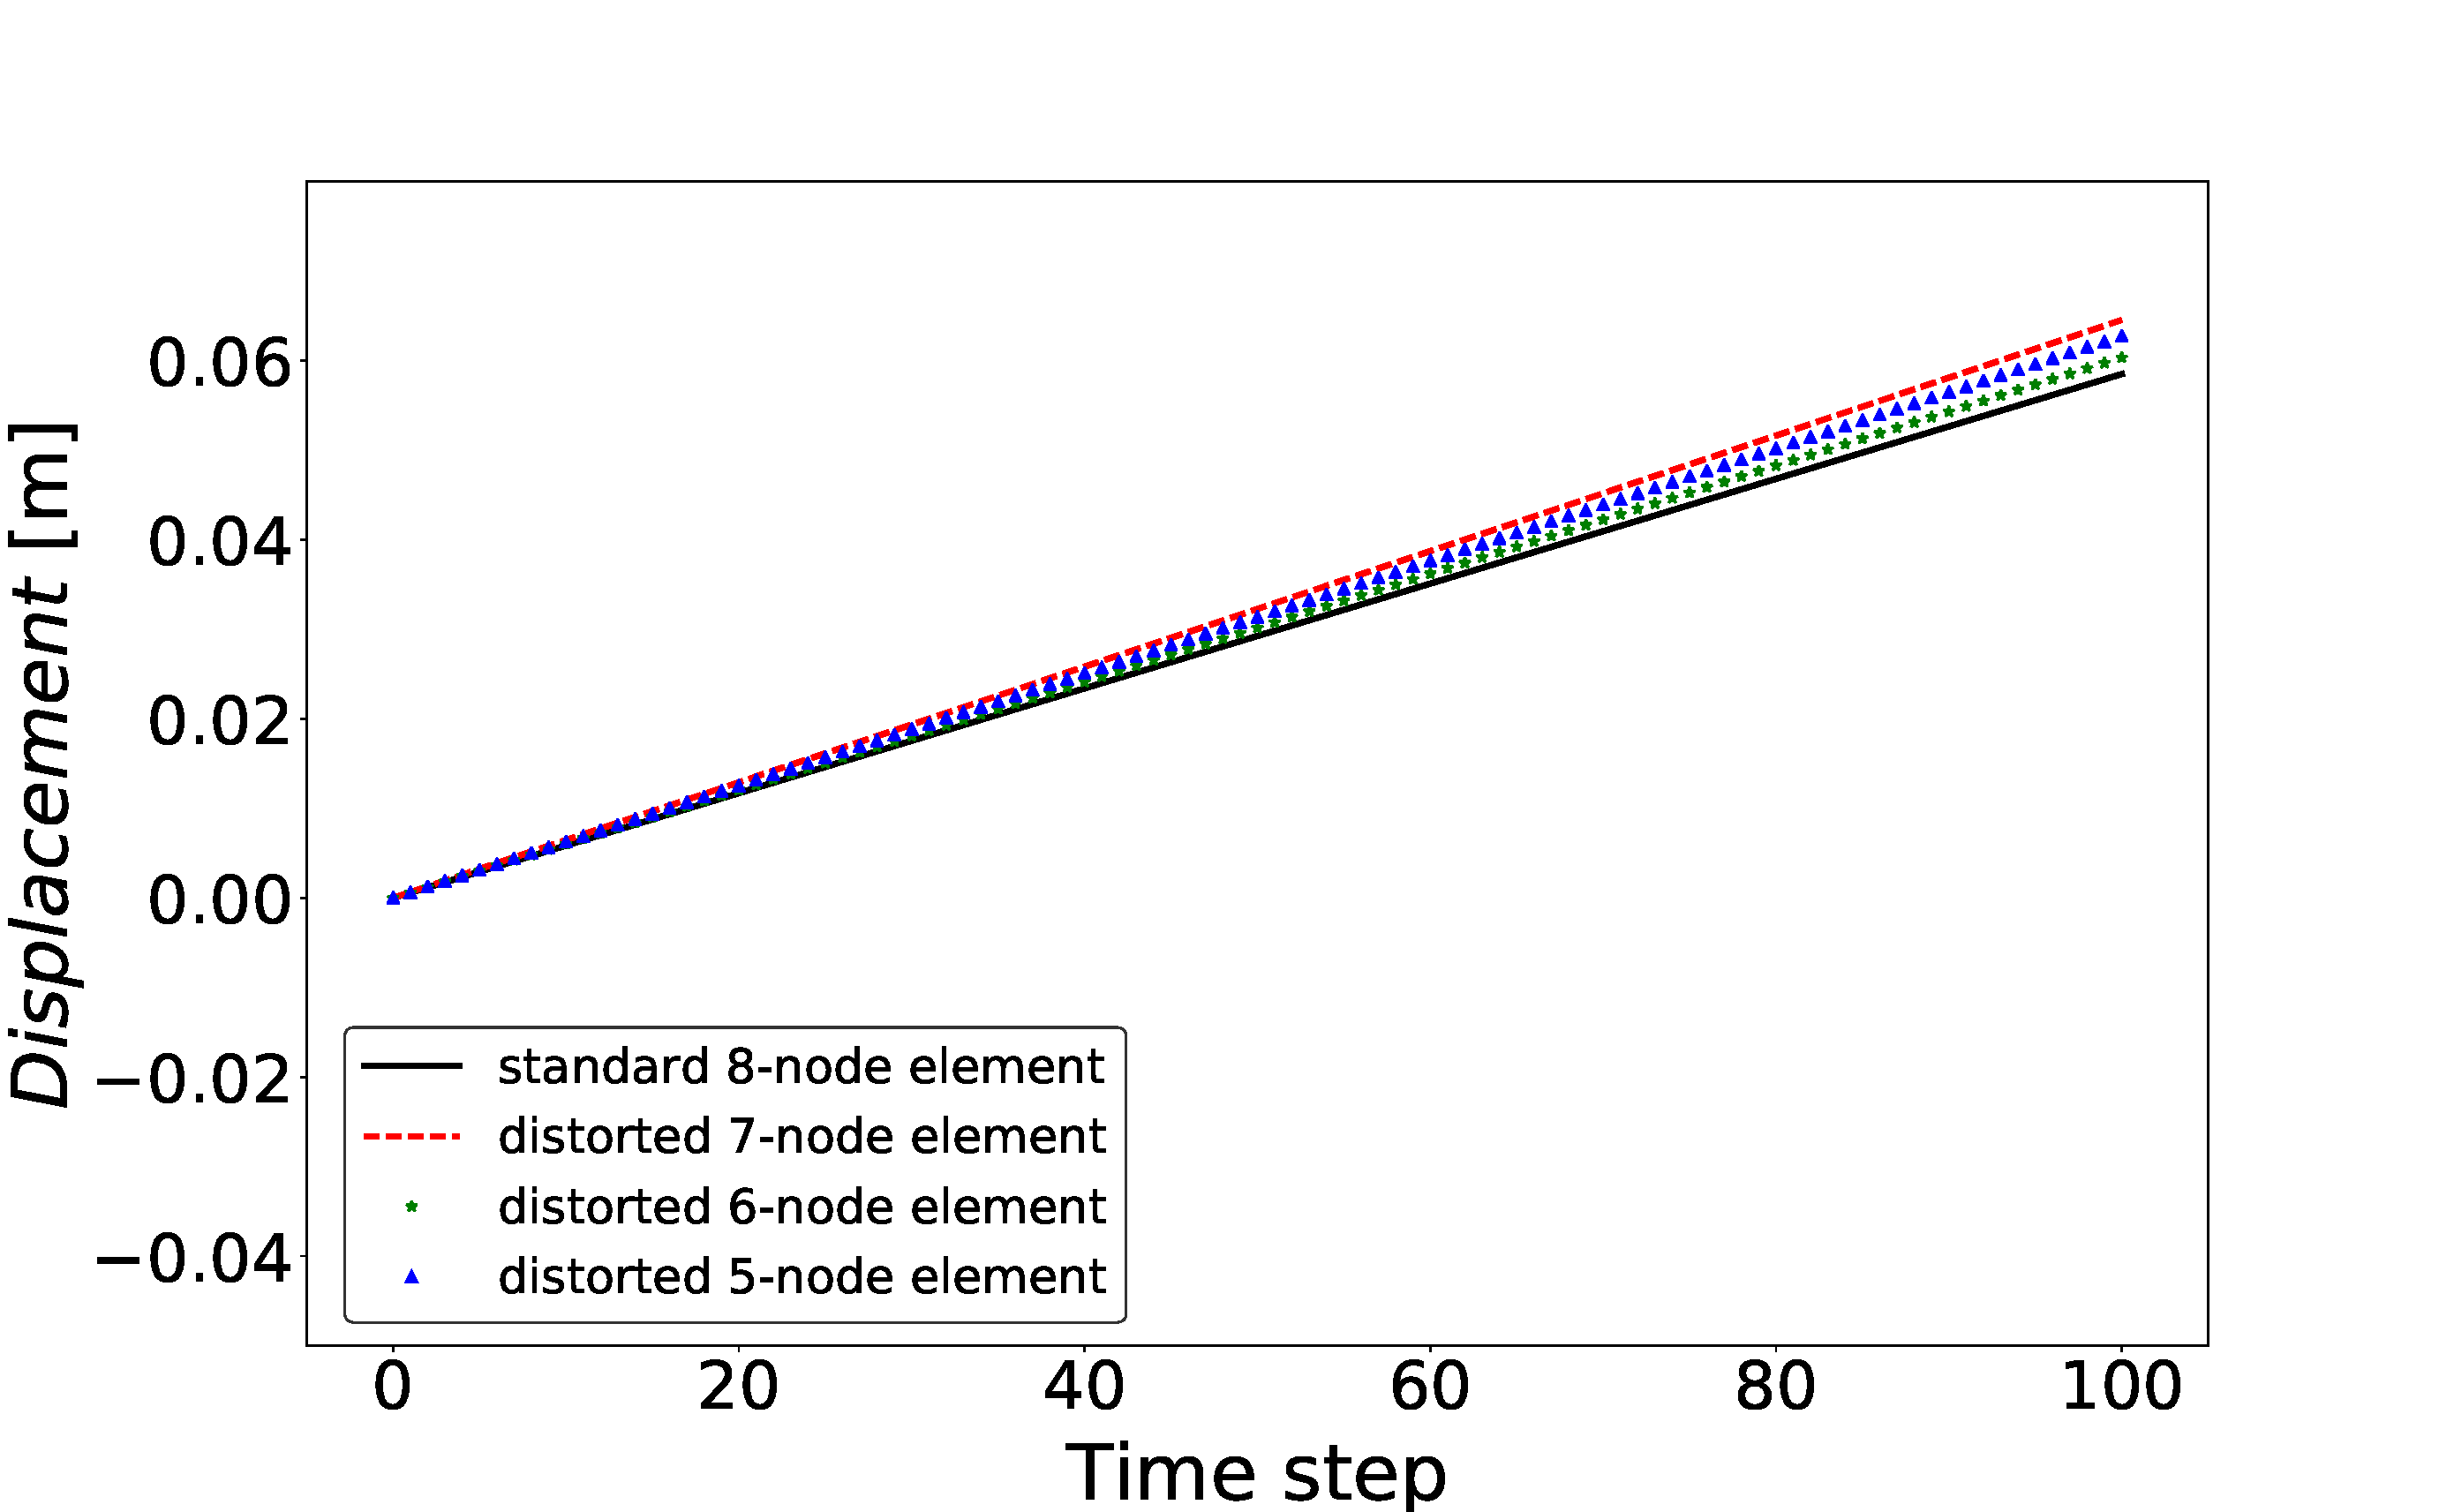
\includegraphics[width=0.8\textwidth]{images/shearing_comparison.pdf}
\end{center}
\caption{\label{Fig: shearing comparison result} Comparison of displacement response under simple shearing}
\end{figure}

\section{Conclusion}

\textbf{SASSI\_converter} can conduct mesh conversion between SASSI and RealESSI. 
%
The strategy of creating dummy ESSI nodes at the same location with different IDs can well handle distorted 7-node, 6-node and 5-node SASSI element. 

%
The accuracy of distorted 6-node element is good enough. 
%
For distorted 5-node element and 7-node element, when the external force is within certain limit, the error is also tolerable; 
%
The prediction error of displacement response grows with the increase of external force. 
%
Although ESSI can deal with these types of special element, as suggested by \citet{Ostadan2007b}, the integration order of these elements should be increased and very distorted elements should be avoided as much as possible.

\bibliographystyle{agsm}
\setlength\bibsep{0.3pt}

\bibliography{./refmech}

\end{document}


